\section{Results}\label{sec:results}
\subsection{Evolution and comparison with the random-search baseline}
The cohort of record ran \gIslands{} evolving islands of \gEvalsIsland{} evaluations each (\gEvalsTotal{} total evaluations) on
\gHost{} from \gStarted{} to \gFinished{} UTC, plus \gBaselineIslands{} scrambled-Sobol random-search control islands
(\gBaselineEvals{} evaluations) under identical tier promotion and scoring. Fig.~\ref{fig:evo} plots the best score of every
island against evaluations, compared with the random-search control. Whereas the \gBaselineIslands{} random-search control
islands reached a best score of \gBaselineBest, \gBeatingBaseline{} of the \gIslands{} evolving islands surpassed that mark
(cohort median rose from \gCohortSobolMed{} after the Sobol start to \gCohortMed). In the winning island (\gWinIsland, which
started at \gScoreSobol{} after its Sobol initialization), the best score on the $h = \gH$~mm search grid reached \gScoreSearch;
the winner of record \gDesign{} was first found at evaluation \gWinFoundEvals{} (\gWinnerSearchScore{} on the $h = \gH$~mm
search grid and \gScore{} at Tier~2 on the $h = \gHRank$~mm ranking grid). Fig.~\ref{fig:lineage} shows the best design of
\gWinIsland{} at each logged checkpoint from a fixed camera.

\begin{figure}[t]
\centering
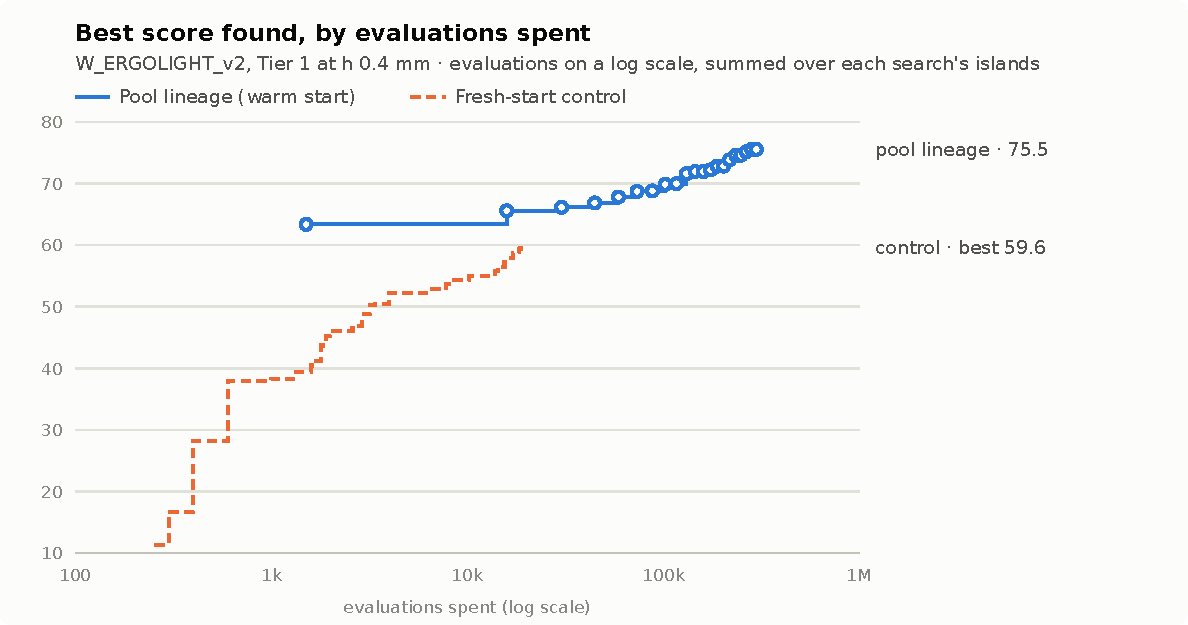
\includegraphics[width=\linewidth]{evolution.pdf}
\caption{Best \code{W\_ERGOLIGHT\_v2} score found against evaluations across all \gIslands{} evolving islands (winning island
\gWinIsland{} highlighted) against the scrambled-Sobol random-search control (\gBaselineBest{} max).}\label{fig:evo}
\end{figure}

\begin{figure*}[t]
\centering
% generated by g5-release-tex: best design of the winning island (v6: of the pool lineage) at each checkpoint
\begin{minipage}[t]{0.196\textwidth}\centering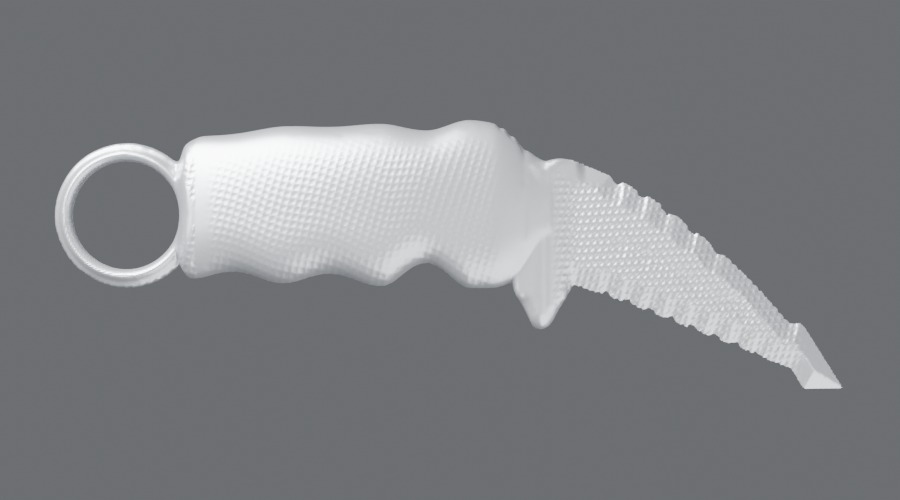
\includegraphics[width=\linewidth]{../../../docs/g5/v6.0.0/img/lineage_epoch00_pool.jpg}\\[-1pt]{\EItablefont pool epoch00/pool\\ 63.36, 103.6 g\\ \textbf{warm start}}\end{minipage}\hfill
\begin{minipage}[t]{0.196\textwidth}\centering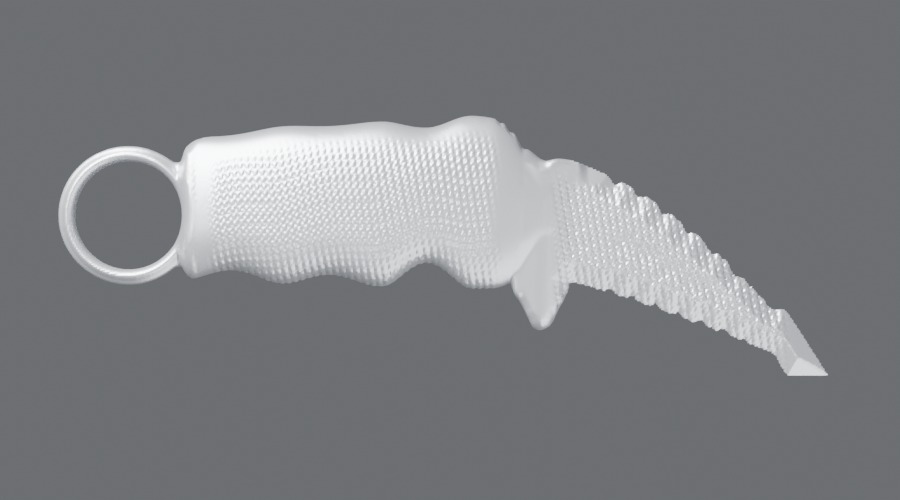
\includegraphics[width=\linewidth]{../../../docs/g5/v6.0.0/img/lineage_p04.jpg}\\[-1pt]{\EItablefont pool pools/p04\\ 67.81, 95.9 g}\end{minipage}\hfill
\begin{minipage}[t]{0.196\textwidth}\centering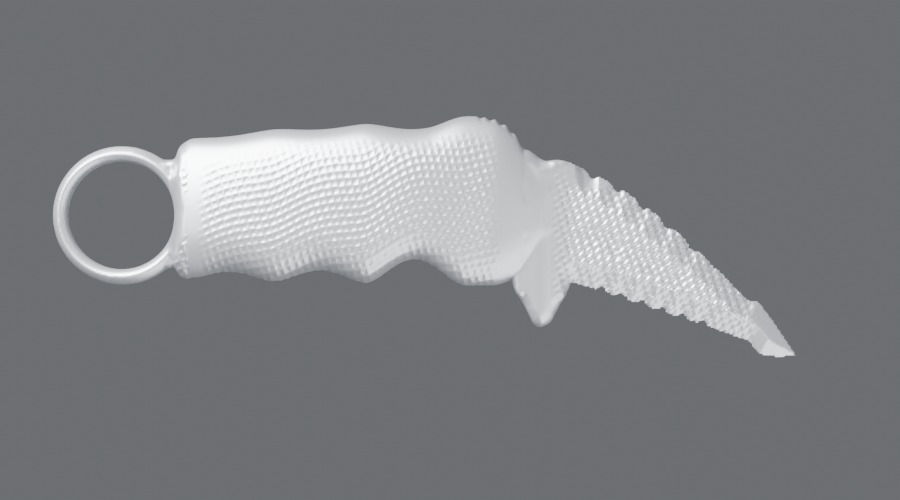
\includegraphics[width=\linewidth]{../../../docs/g5/v6.0.0/img/lineage_p10.jpg}\\[-1pt]{\EItablefont pool pools/p10\\ 71.94, 96.2 g}\end{minipage}\hfill
\begin{minipage}[t]{0.196\textwidth}\centering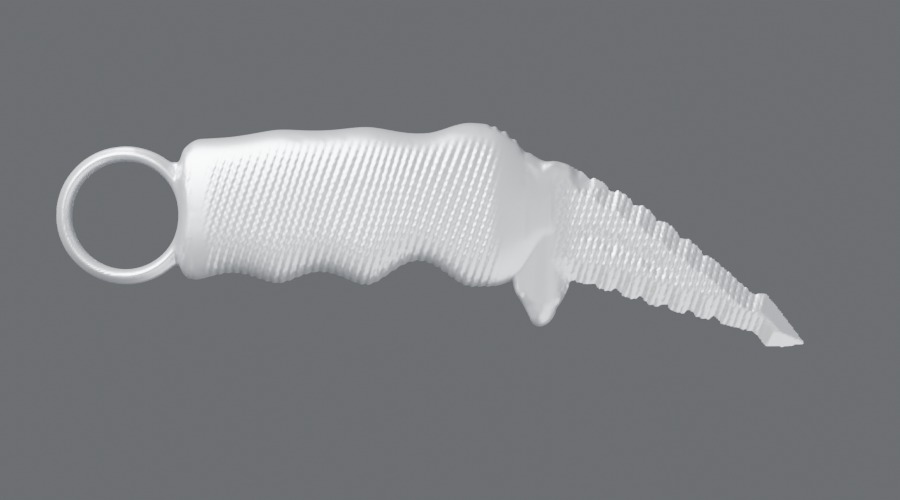
\includegraphics[width=\linewidth]{../../../docs/g5/v6.0.0/img/lineage_p14.jpg}\\[-1pt]{\EItablefont pool pools/p14\\ 72.81, 90.7 g}\end{minipage}\hfill
\begin{minipage}[t]{0.196\textwidth}\centering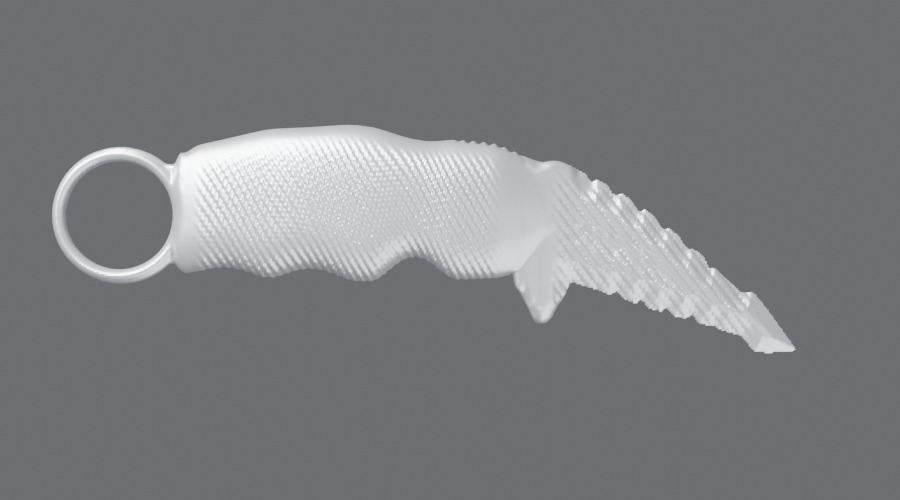
\includegraphics[width=\linewidth]{../../../docs/g5/v6.0.0/img/lineage_p20.jpg}\\[-1pt]{\EItablefont pool pools/p20\\ 75.54, 88.6 g\\ \textbf{final pool}}\end{minipage}\hfill

\caption{Best design of \gWinIsland{} at each logged checkpoint: evaluation count, \code{W\_ERGOLIGHT\_v2} score, and mass on
the search grid. Fixed camera, lighting and material across all frames.}\label{fig:lineage}
\end{figure*}

\subsection{Grid check and final Tier-2 ranking}
To verify grid independence, the top designs were evaluated across five voxel pitches $h \in \{0.4, 0.3, 0.25, 0.2, 0.15\}$~mm
(Table~\ref{tab:grid}). With smoothed-Heaviside partial-volume integration and width-aware drainage, the $0.20$~mm and
$0.15$~mm grids agree within \gGridAgree\,\%, and the search's $0.40$~mm mass matches the $0.20$~mm mass of record within
\gGridSpanPct\,\%. Table~\ref{tab:top} lists the top designs from the final Tier-2 ranking (shortlist \gShortlist) at
$h = \gHRank$~mm and $0.08~\mathrm{mm^2}$ solid-tip mesh resolution; the top eight rows span \gScore--\gTopLast. Re-ranking
the shortlist at Tier~2 is essential: the search-grid leader \gSearchLeaderId{} (\gSearchLeaderTierOne{} at Tier~1, where the 1D
section model estimated tip axial SF~\gSearchLeaderTipSecAx) drops to rank~\gSearchLeaderRank{} at Tier~2 (\gSearchLeaderTierTwo)
because its 3D \code{TET10} solid-tip submodel carries the $\gReqTipAxN$~N axial case at SF~\gSearchLeaderTipSolAx{} (margin
$v = \gSearchLeaderMargin$ against the $\gReqSfYield$ requirement).

\begin{table}[t]
\caption{Grid check: partial-volume mass (g) of the top designs across five voxel pitches $h$ (mm)}\label{tab:grid}
\centering
\begin{tabular}{@{}lrrrrr@{}}
\toprule
Design & 0.4 & 0.3 & 0.25 & 0.2 & 0.15 \\
\midrule
\gGridRows
\bottomrule
\end{tabular}
\end{table}

\begin{table}[t]
\caption{Final ranking: Tier 2 at $h = \gHRank$ mm and $0.08~\mathrm{mm^2}$ solid-tip mesh}\label{tab:top}
\centering
\begin{tabular}{@{}rlrrr@{}}
\toprule
Rank & Design & Score & $W$ & Mass (g) \\
\midrule
\gTopEightRows
\bottomrule
\end{tabular}
\end{table}

\begin{figure*}[t]
\centering
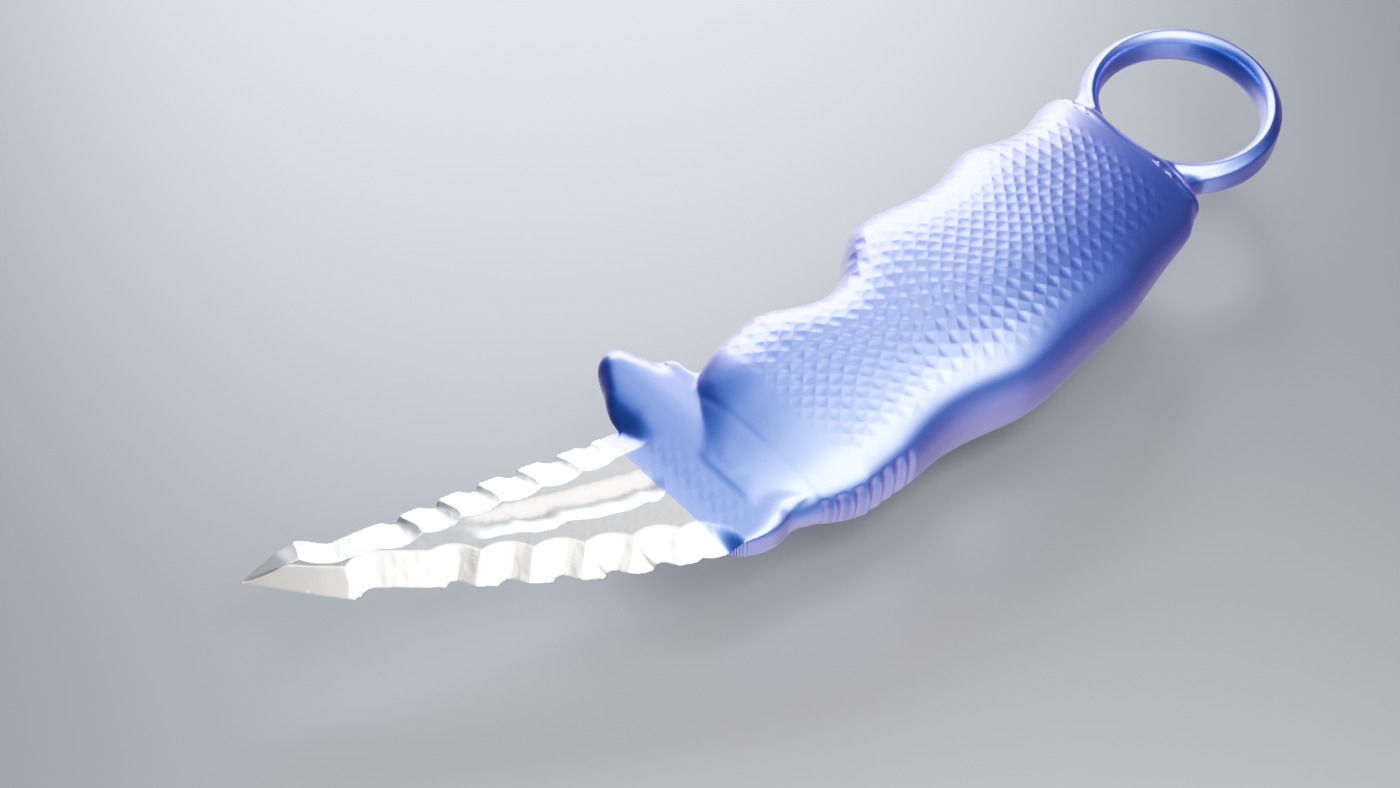
\includegraphics[width=0.49\textwidth]{hero.jpg}\hfill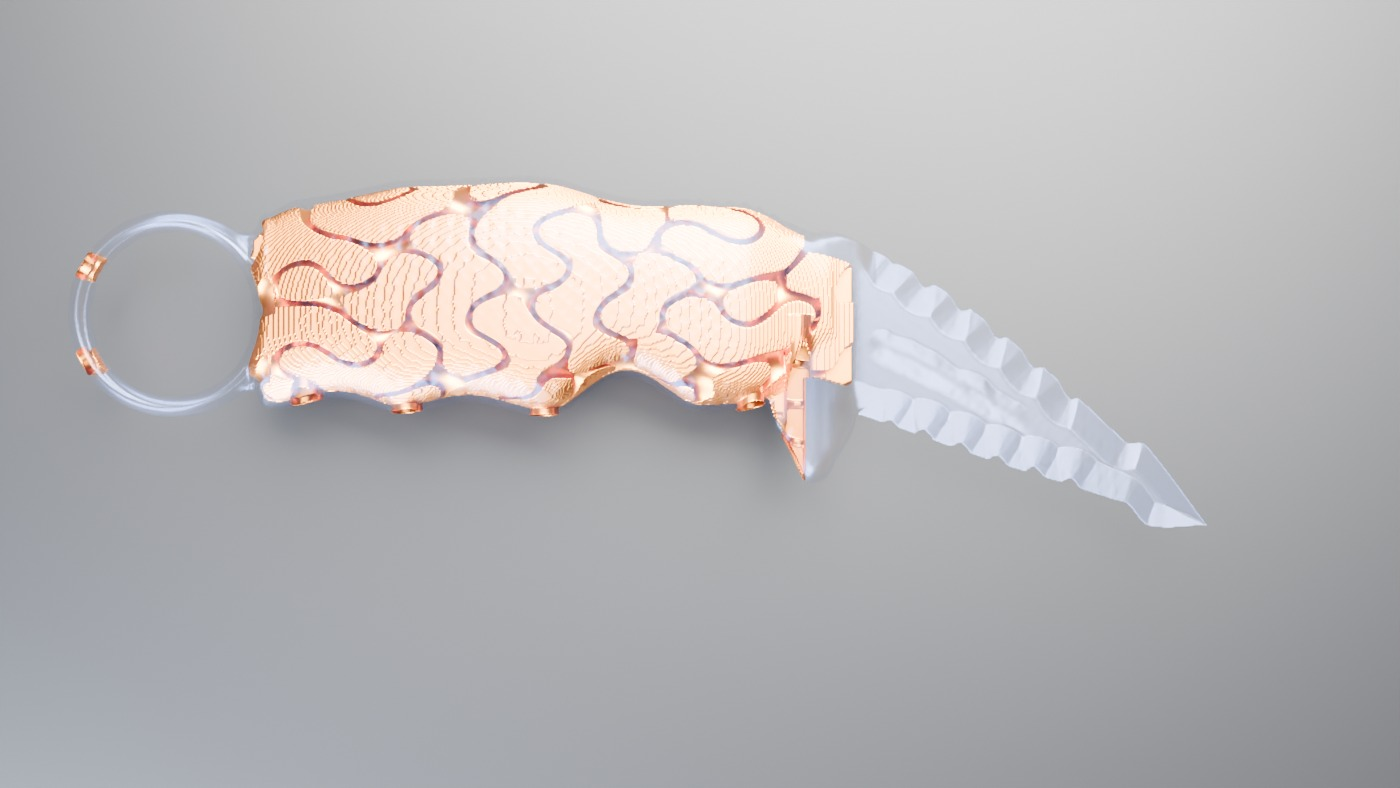
\includegraphics[width=0.49\textwidth]{xray.jpg}\\[3pt]
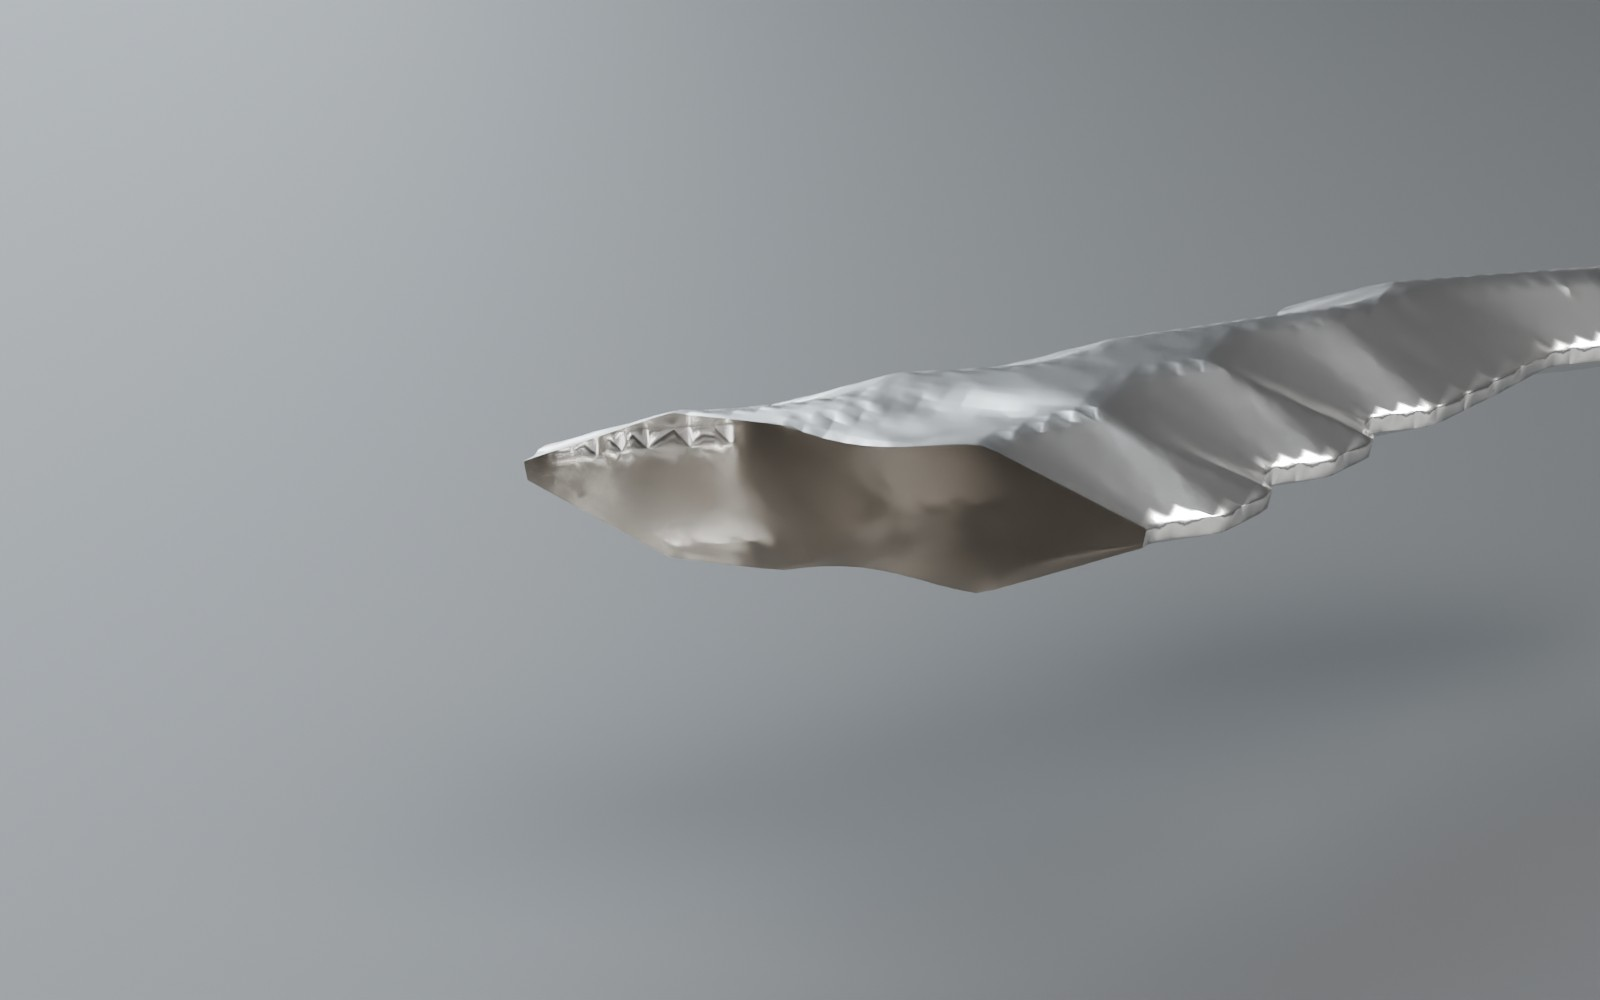
\includegraphics[width=0.32\textwidth]{cut_b.jpg}\hfill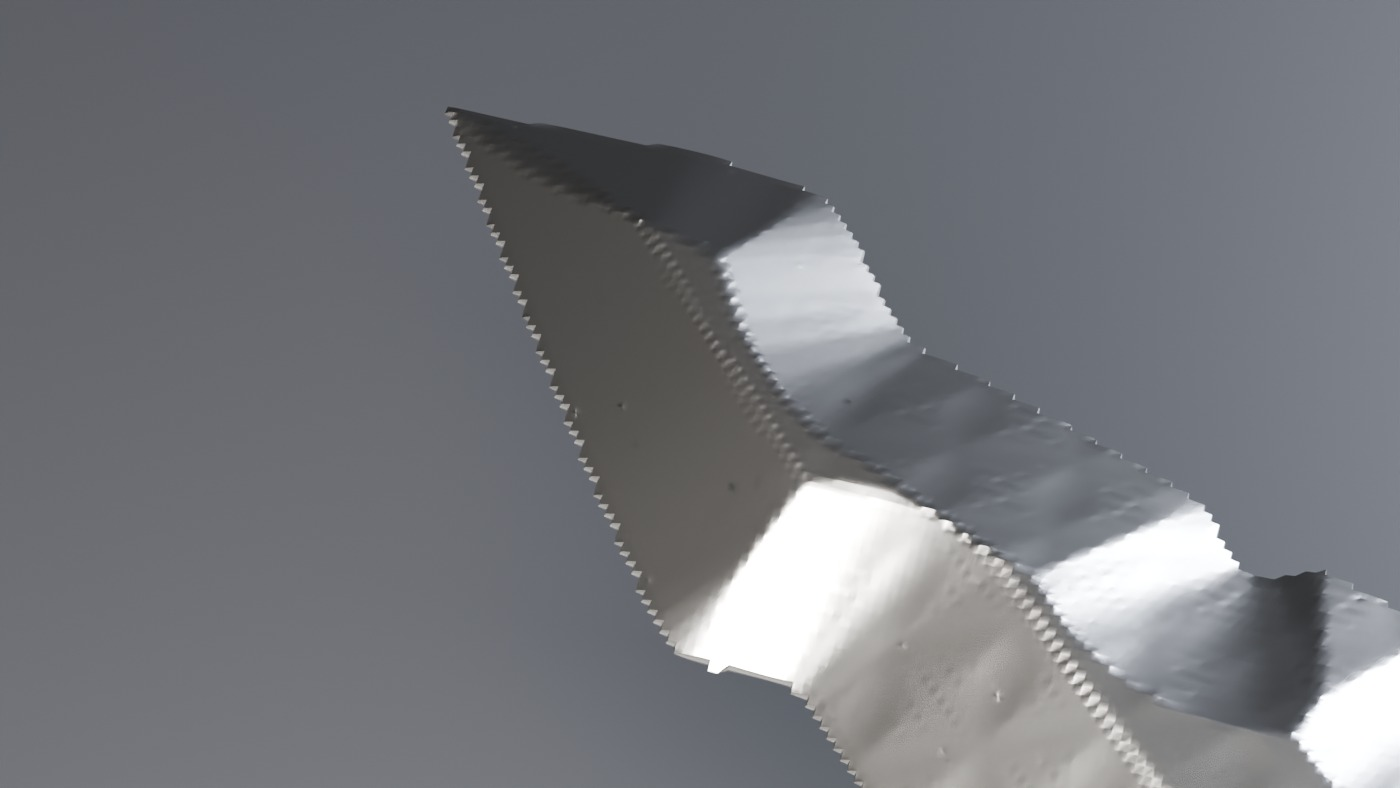
\includegraphics[width=0.32\textwidth]{tip.jpg}\hfill
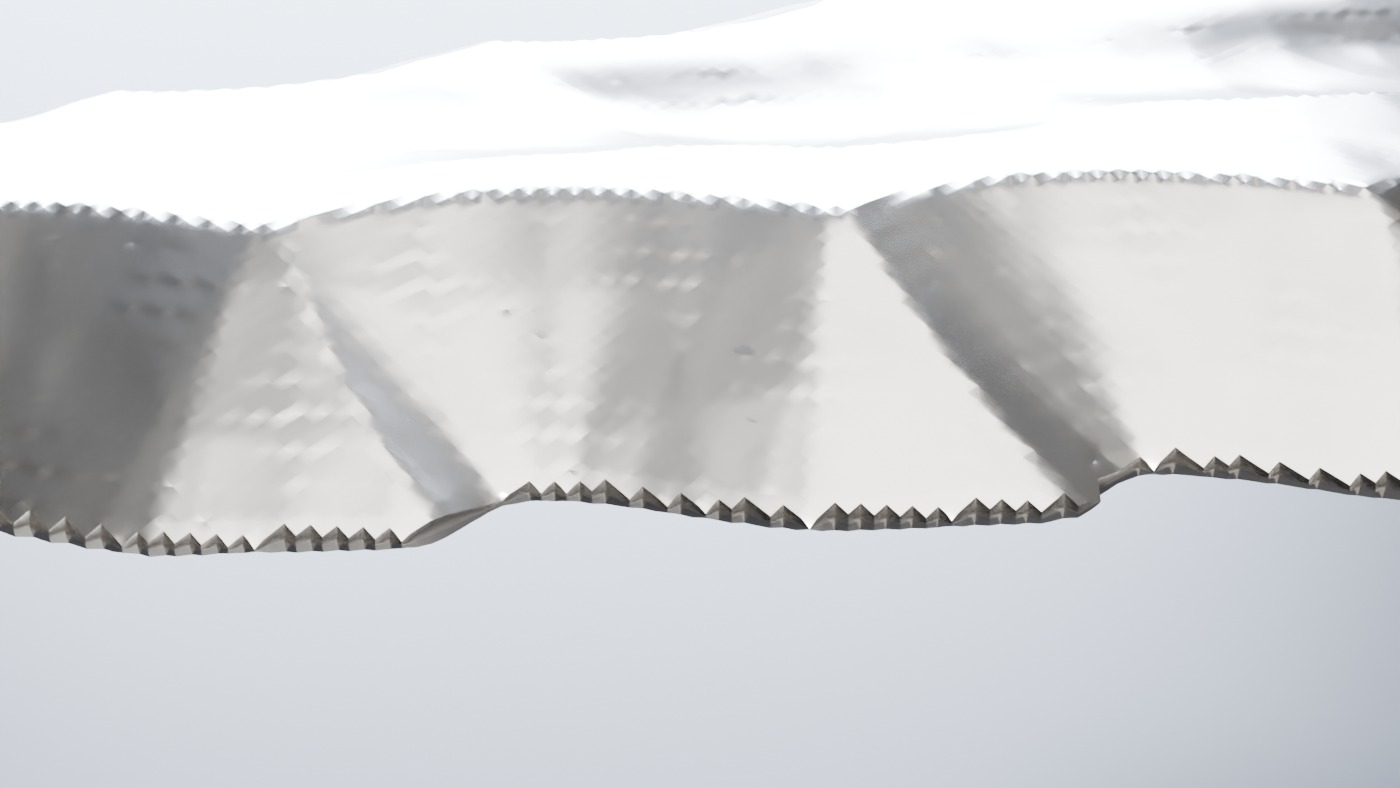
\includegraphics[width=0.32\textwidth]{edge_b.jpg}
\caption{\gDesign. Top: three-quarter view as decoded (before grinding), and an x-ray cutaway showing the internal sheet-TPMS
cavities and rib-clear drainage ports in amber. Bottom: cross-section across the blade 30~mm from the point, the sharp point
wedge, and the spine edge with its rounded-gullet serrations, as decoded (before grinding).}\label{fig:hero}
\end{figure*}

\subsection{The best individual (\gDesign)}
The winning individual, \gDesign{} (genome hash \gGenomeSha), scores \gScore{} under \code{W\_ERGOLIGHT\_v2} with weighted base
\gBase, ergonomic multiplier $E = \gE$ ($E^5 = \gEFive$), and worst-margin multiplier $W = \gW$ (worst safety-factor ratio
$\mu = \gWorstMarginRatio$ on \gWorstMarginCase). Its finished partial-volume mass of record at $h = \gHRank$~mm is
\gMassFinishedG{}~g (\gMassG{}~g on the watertight print mesh; solid outer envelope \gVolEnv{}~$\mathrm{mm^3}$, \gMassEnvG{}~g).
Its grip is \gLg{}~mm long with a swell perimeter of \gSwellPerim{}~mm ($84$--$100$~mm target band) and height-to-thickness ratio
\gHoT{} ($1.5$--$1.8$ target band); the guard is \gGuardH{}~mm high and the straight-line blade reach is \gReach{}~mm. Internal
sealed void volume is \gSealedVoid{}~$\mathrm{mm^3}$ (open surface crevices \gCreviceVoid{}~$\mathrm{mm^3}$), drained through
\gPortCount{} ports of diameter \gPortD{}~mm. Because the genome scopes the evolved surface texture onto the blade
(\code{scope\_blade} $= \gScopeBlade$, depth $\gTexAmp$~mm, pitch $\gTexPitch$~mm), the as-decoded renders and print meshes show
knurling across the blade flats and bevels; the analytical edge cross-sections (Fig.~\ref{fig:edges}) and edge metrics evaluate
the bevel law restored after post-build grinding ($\gReqEdgeFinishMm$~mm finishing allowance per ground face). Fig.~\ref{fig:hero}
and Fig.~\ref{fig:edges} show its geometry;
Table~\ref{tab:best} reports all 16 structural load cases and key geometric measurements against \code{RS-karambit-v5}.

\begin{table}[t]
\caption{Measurements and safety factors of the best individual \gDesign{} against \code{RS-karambit-v5}}\label{tab:best}
\centering
\EItablefont
\setlength{\tabcolsep}{2.2pt}
\begin{tabular}{@{}lrrr@{}}
\toprule
Quantity / Load case & Value & Req. & $v$ \\
\midrule
Score (\code{W\_ERGOLIGHT\_v2}) & \gScore & --- & $E=\gE$ \\
Mass, partial vol.\ / mesh (g) & \gMassFinishedG{} / \gMassG & $\gReqMassGoal$ goal ($\le \gReqMassCeil$) & $W=\gW$ \\
Sealed void ($\mathrm{mm^3}$) / ports & \gSealedVoid{} / $\varnothing\gPortD$ & $0$ / $\ge \gReqPortD$ & $N=\gPortCount$ \\
Grip $L_g$ / perim.\ (mm) / $H/T$ & \gLg{} / \gSwellPerim{} / \gHoT & $\ge \gReqLg$ / $\gReqPerimMin$--$\gReqPerimMax$ & $\gReqHoTMin$--$\gReqHoTMax$ \\
Guard $h$ / CoM to choil (mm) & \gGuardH{} / \gComIdx & $\ge \gReqGuardH$ / $\le \gReqComIdx$ & --- \\
Point angle $1$ / $3$~mm (\textdegree) & \gPointAngleOne{} / \gPointAngleThree & $\le \gReqPtOne$ / $\le \gReqPtThree$ & $w_2=\gPointWidthTwo$ \\
Edge A / B grind (\textdegree, max \gEdgeMaxAngle) & \gEdgeAAngle{} / \gEdgeBAngle & $\gReqEdgeMin$--$\gReqEdgeMax^\circ$ & flat \gEdgeMaxApex \\
Serr.\ depth (mm), scallops A / B & \gEdgeADepth{} (\gEdgeATeeth) / \gEdgeBDepth{} (\gEdgeBTeeth) & $\gReqSerrMin$--$\gReqSerrMax$, $\ge \gReqScallopsMin$ & $r_g \ge \gReqGulletR$ \\
\midrule
Lateral limit ($\gReqLatLimNm$~N$\cdot$m, plate) & SF \gLoadLatLim & $\ge \gReqSfYield$ & \gMarginLatLim \\
Lateral ult.\ ($\gReqLatUltNm$~N$\cdot$m, plate) & SF \gLoadLatUlt & $\ge \gReqSfUlt$ & \gMarginLatUlt \\
Body twist ($\gReqTwistLimNm$~N$\cdot$m, plate) & SF \gLoadTwistLim & $\ge \gReqSfYield$ & \gMarginTwistLim \\
Tip axial ($\gReqTipAxN$~N, \code{TET10}) & SF \gLoadTipAxial & $\ge \gReqSfYield$ & \gMarginTipAxial \\
Tip lateral ($\gReqTipLatN$~N, \code{TET10}) & SF \gLoadTipLat & $\ge \gReqSfYield$ & \gMarginTipLat \\
Tip twist ($\gReqTipTwNm$~N$\cdot$m, \code{TET10}) & SF \gLoadTipTwist & $\ge \gReqSfYield$ & \gMarginTipTwist \\
Grip squeeze ($\gReqGripSqN$~N) & SF \gLoadGripSqueeze & $\ge \gReqSfYield$ & \gMarginGripSqueeze \\
Guard slip push ($\gReqGuardPushN$~N) & SF \gLoadGuardPush & $\ge \gReqSfYield$ & \gMarginGuardPush \\
Ring bearing ($\gReqRingBearN$~N, $\pm \gReqRingArcDeg^\circ$) & SF \gLoadRingBear & $\ge \gReqSfRing$ & \gMarginRingBear \\
Ring back ($\gReqRingBackN$~N) & SF \gLoadRingBack & $\ge \gReqSfRing$ & \gMarginRingBack \\
Ring in-plane sweep ($\gReqRingAnyN$~N) & SF \gLoadRingAny & $\ge \gReqSfYield$ & \gMarginRingAny \\
Axial pull ($\gReqPullN$~N, plate/grip) & SF \gLoadPull & $\ge \gReqSfYield$ & \gMarginPull \\
Serration teeth ($\gReqSnagN/\gReqPryN$~N, all) & SF \gLoadTeeth & $\ge \gReqSfYield$ & \gMarginTeeth \\
Fatigue ($10^6$ cyc, FKM class) & SF \gLoadFatigue & $\ge \gReqSfFat$ & \gMarginFatigue \\
Yield sequence ($\min$ per case) & \gLoadSeqMin & $\ge \gReqSeqRatio$ & \gMarginSeq \\
Tip buckling $\lambda$ ($\gReqTipAxN$~N, Ritz) & \gLoadBuckling & $\ge \gReqBuckling$ & \gMarginBuckling \\
\bottomrule
\end{tabular}
\end{table}

\begin{table}[t]
\caption{Verification studies (\code{evidence/g5/v\gRecord/vv/} and \code{release.json}): plate refinement, solid-tip
refinement and solver checks}\label{tab:vv}
\centering
\EItablefont
\setlength{\tabcolsep}{2.4pt}
\begin{tabular}{@{}llrrr@{}}
\toprule
Study & Quantity & Coarse & Med. & Fine \\
\midrule
Plate ($1.2/0.3/0.15~\mathrm{mm^2}$) & Lat.\ limit SF & \gVvPlateLatA & \gVvPlateLatB & \gVvPlateLatC \\
Plate ($1.2/0.3/0.15~\mathrm{mm^2}$) & Twist limit SF & \gVvPlateTwistA & \gVvPlateTwistB & \gVvPlateTwistC \\
Tip \code{TET10} (sec/$0.15/0.08$) & Axial SF & \gVvTipAxA & \gVvTipAxB & \gVvTipAxC \\
Tip \code{TET10} (sec/$0.15/0.08$) & Lateral SF & \gVvTipLatA & \gVvTipLatB & \gVvTipLatC \\
Tip \code{TET10} (sec/$0.15/0.08$) & Twist SF & \gVvTipTwA & \gVvTipTwB & \gVvTipTwC \\
Tier-1 determinism & Archive rows & \gCohortElites & --- & \gTierOneReproduced{} exact \\
Linux \code{x86\_64} Tier 2 & Max rel.\ diff & \gLinuxDesigns{} top & --- & \gLinuxMaxRelDiff \\
Ritz vs.\ Euler column & $|\Delta P_\mathrm{cr}|/P_\mathrm{cr}$ & --- & --- & \gVvRitzErr \\
\bottomrule
\end{tabular}
\end{table}

\begin{figure}[!t]
\centering
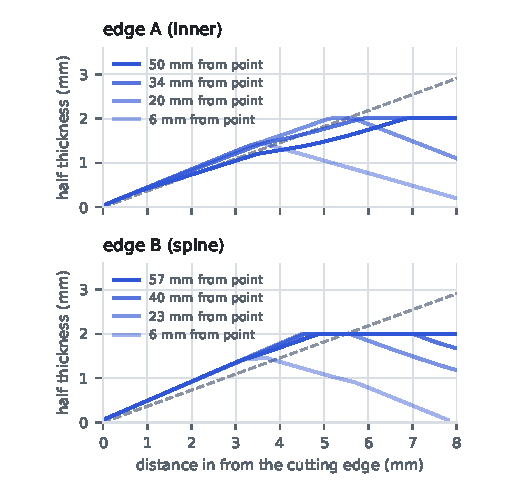
\includegraphics[width=\linewidth]{edge_sections.pdf}
\caption{Upper half of the blade cross-section at four stations along each edge of \gDesign, true scale, measured normal to
the serrated edge from the exact decoder law (dashed: $\gReqEdgeMin^\circ$ per side, the requirement's minimum).}\label{fig:edges}
\end{figure}
